% =============================================================================
% Présentation Beamer — Lecture de texte dans l'espace public (malvoyants)
% Compilation (depuis docs/presentation/) :   latexmk -pdf presentation.tex
% Tableaux, figures et chiffres : results/benchmark/ (scripts/benchmark.py)
% =============================================================================
\documentclass[aspectratio=169,11pt]{beamer}

\usepackage[utf8]{inputenc}
\usepackage[T1]{fontenc}
\usepackage{lmodern}
\usepackage[french]{babel}
\usepackage{booktabs}
\usepackage{graphicx}
\usepackage{tikz}
\usetikzlibrary{arrows.meta,positioning}

\graphicspath{{../figures/}{../../results/benchmark/}}
% Styles TikZ définis ici : le « #1 » est interdit dans le corps d'une frame
\tikzset{bloc/.style={draw, rounded corners=3pt, minimum width=2.15cm, minimum height=1.3cm,
  align=center, font=\small, fill=#1}, bloc/.default=gray!8,
  fleche/.style={-{Stealth[length=2.2mm]}, thick}}

% --- Thème sobre, contrasté (cohérent avec le sujet : la lisibilité) ---------
\usetheme{default}
\definecolor{encre}{HTML}{1B2A41}
\definecolor{accent}{HTML}{C44E52}
\definecolor{doux}{HTML}{5B6B80}
\setbeamercolor{frametitle}{fg=white,bg=encre}
\setbeamercolor{title}{fg=encre}
\setbeamercolor{structure}{fg=accent}
\setbeamercolor{normal text}{fg=encre}
\setbeamerfont{frametitle}{series=\bfseries,size=\large}
\setbeamertemplate{frametitle}{\nointerlineskip\begin{beamercolorbox}[wd=\paperwidth,ht=2.4ex,dp=1.2ex,leftskip=1em]{frametitle}\insertframetitle\end{beamercolorbox}}
\setbeamertemplate{navigation symbols}{}
\setbeamertemplate{footline}{\hfill{\scriptsize\color{doux}\insertframenumber/\inserttotalframenumber}\hspace{1em}\vspace{0.6em}}
\setbeamertemplate{itemize items}[circle]
% Légendes des tableaux masquées : trop longues pour des diapositives (voir le rapport)
\setbeamertemplate{caption}{}

\IfFileExists{../../results/benchmark/chiffres.tex}{% Généré par scripts/benchmark.py — ne pas modifier à la main
\newcommand{\nbImages}{50}
\newcommand{\configFinale}{etape4\_v2 : mser + otsu}
\newcommand{\baseFmed}{0{,}013}
\newcommand{\baseFmoy}{0{,}086}
\newcommand{\basePmed}{0{,}007}
\newcommand{\baseRmed}{0{,}120}
\newcommand{\baseCERmed}{6{,}59}
\newcommand{\finFmed}{0{,}281}
\newcommand{\finFmoy}{0{,}326}
\newcommand{\finFicBas}{0{,}12}
\newcommand{\finFicHaut}{0{,}41}
\newcommand{\finPmed}{0{,}250}
\newcommand{\finRmed}{0{,}400}
\newcommand{\finCERmed}{0{,}67}
\newcommand{\finMieux}{32}
\newcommand{\finEgal}{14}
\newcommand{\finPire}{4}
\newcommand{\finP}{$<$\,0{,}001}
\newcommand{\facteurF}{21}
\newcommand{\basePsmTroisFmed}{0{,}000}
}{%
  \newcommand{\nbImages}{?}\newcommand{\configFinale}{?}\newcommand{\baseFmed}{?}%
  \newcommand{\basePmed}{?}\newcommand{\baseRmed}{?}\newcommand{\finFmed}{?}%
  \newcommand{\finFicBas}{?}\newcommand{\finFicHaut}{?}\newcommand{\finPmed}{?}%
  \newcommand{\finRmed}{?}\newcommand{\finMieux}{?}\newcommand{\finEgal}{?}%
  \newcommand{\finPire}{?}\newcommand{\finP}{?}\newcommand{\facteurF}{?}}
\newcommand{\tableauOuNote}[2]{\IfFileExists{../../results/benchmark/#1}{\input{../../results/benchmark/#1}}{\textit{#2}}}
\newcommand{\gros}[1]{{\Large\bfseries\color{accent}#1}}

\title{Assistance à la lecture d'informations\\dans l'espace public pour les personnes malvoyantes}
\subtitle{Détection et reconnaissance de texte dans des scènes urbaines}
\author{Zitouni Zaid, Zerrif Haitam, Zbayar Ziad}
\date{Novembre 2026}

\begin{document}

\begin{frame}[plain]
\titlepage
\end{frame}

% -----------------------------------------------------------------------------
\begin{frame}{Le problème}
\begin{columns}[T]
\column{0.55\textwidth}
\begin{itemize}
\item Nom de rue, numéro, direction, commerce : des informations \alert{conçues pour être vues}
\item L'OCR fonctionne bien sur des documents : fond blanc, texte noir, lignes droites
\item Une photo de rue n'a aucune de ces propriétés :
  \begin{itemize}
  \item texte minoritaire, entouré de feuillage, briques, voitures
  \item ombres, contre-jour, nuit
  \item polarité variable, polices et perspectives variées
  \end{itemize}
\end{itemize}
\column{0.42\textwidth}
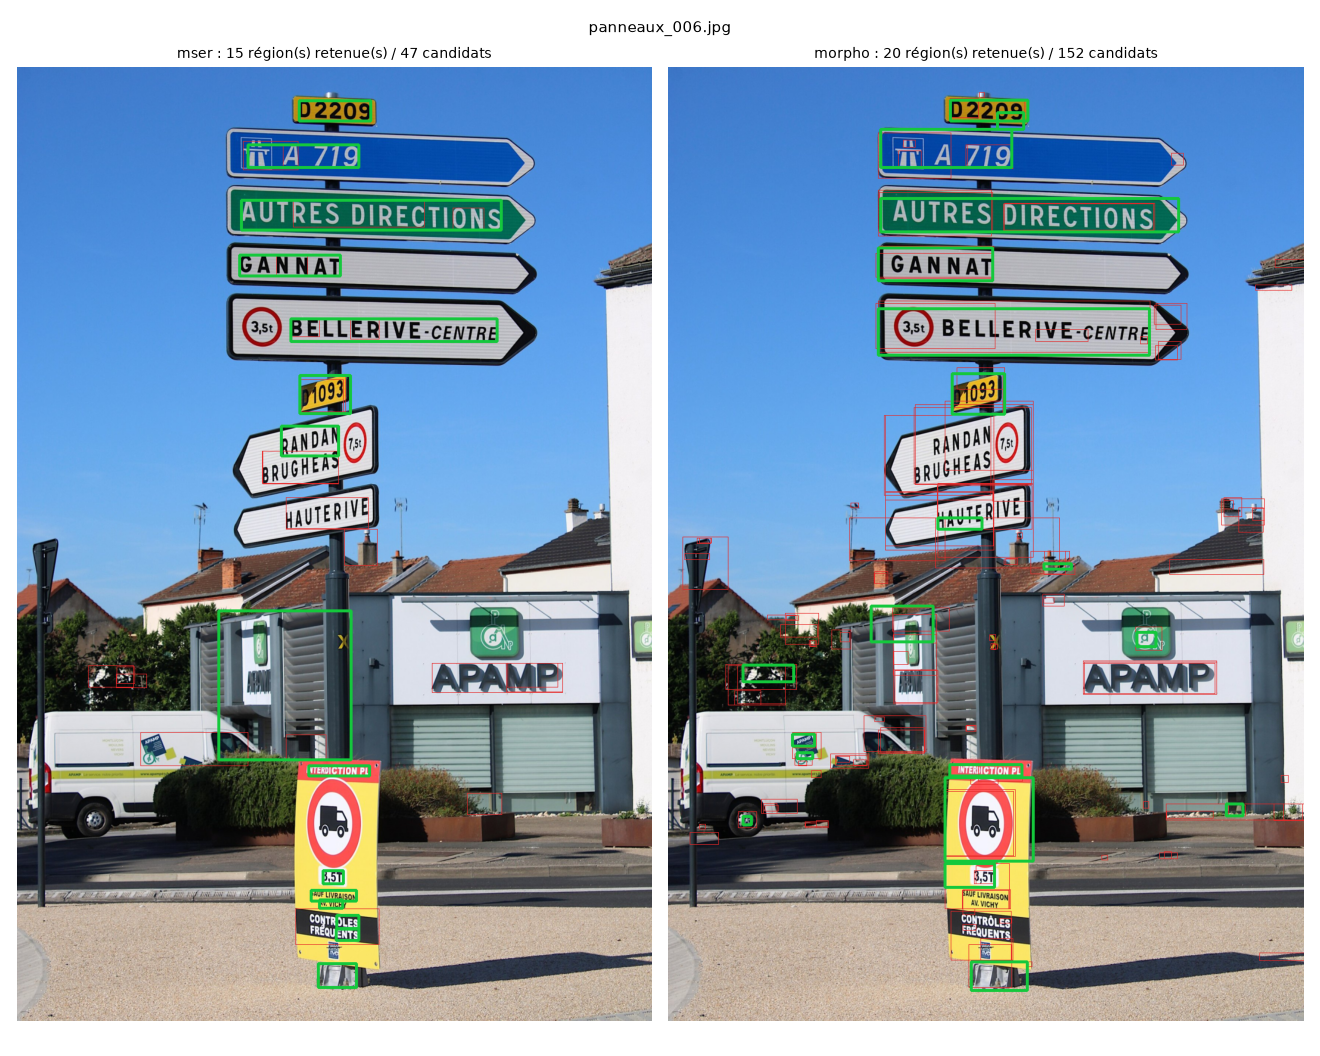
\includegraphics[width=\linewidth]{detection_006.png}
\end{columns}
\vfill
\textbf{Objectif :} photo $\rightarrow$ texte restitué de façon accessible, avec Python, OpenCV, NumPy, SciPy, Matplotlib et Tesseract.
\end{frame}

% -----------------------------------------------------------------------------
\begin{frame}{Les données : \nbImages{} photographies annotées}
\begin{columns}[T]
\column{0.5\textwidth}
\begin{itemize}
\item Source : \alert{Wikimedia Commons}, licences libres seulement (CC0, CC BY, CC BY-SA)
\item Auteur et licence de chaque image tracés dans \texttt{SOURCES.csv}
\item Scènes françaises et marocaines, dont de la signalisation bilingue
\item Vérité terrain : le texte exact, une ligne par ligne
\item Règle : \emph{tout texte de signalétique lisible} (hors plaques d'immatriculation)
\end{itemize}
\column{0.45\textwidth}
\centering
\begin{tabular}{lr}
\toprule
Catégorie & Images \\
\midrule
plaques de rue & 35 \\
panneaux & 7 \\
affiches, enseignes & 5 \\
numéros & 3 \\
\midrule
total & 50 \\
\bottomrule
\end{tabular}
\end{columns}
\end{frame}

% -----------------------------------------------------------------------------
\begin{frame}{Architecture : un pipeline modulaire}
\centering
\begin{tikzpicture}
\node[bloc] (a) {1. Acquisition\\\scriptsize gris, 1600 px};
\node[bloc=blue!8, right=0.4cm of a] (p) {2. Prétraitement\\\scriptsize débruitage,\\\scriptsize contraste};
\node[bloc=green!10, right=0.4cm of p] (l) {4. Localisation\\\scriptsize MSER,\\\scriptsize morphologie};
\node[bloc=green!10, right=0.4cm of l] (o) {3+5. Binarisation\\\scriptsize + OCR\\\scriptsize par région};
\node[bloc, right=0.4cm of o] (r) {6. Restitution\\\scriptsize accessible};
\node[bloc=red!8, below=0.8cm of o] (e) {7. Évaluation};
\draw[fleche] (a) -- (p); \draw[fleche] (p) -- (l); \draw[fleche] (l) -- (o); \draw[fleche] (o) -- (r);
\draw[fleche, dashed] (o) -- (e);
\end{tikzpicture}
\vfill
\begin{itemize}
\item Un module par étape, des méthodes \alert{interchangeables par leur nom} : comparaisons systématiques
\item Reproductible : versions figées (\texttt{uv.lock}), image Docker avec Tesseract
\item Piège découvert : le MSER d'OpenCV 5.0 ne détecte \alert{rien} $\Rightarrow$ OpenCV 4 imposé
\end{itemize}
\end{frame}

% -----------------------------------------------------------------------------
\begin{frame}{Comment mesurer ?}
\begin{itemize}
\item \textbf{CER / WER} : distance de Levenshtein, en caractères / en mots
  \begin{itemize}\item non bornés : chaque caractère \emph{inventé} compte\end{itemize}
\item \textbf{Précision, rappel, F1 des mots}, sans tenir compte de l'ordre :
\[ P = \frac{|R\cap H|}{|H|}\qquad \text{Rappel} = \frac{|R\cap H|}{|R|}\qquad F_1=\frac{2PR}{P+R} \]
  \begin{itemize}
  \item \alert{rappel} : quelle part de l'information affichée m'est restituée ?
  \item \alert{précision} : puis-je me fier à ce qui est lu ?
  \end{itemize}
\item \textbf{Statistiques} : médianes, IC à 95\,\% par bootstrap, test apparié de Wilcoxon contre la baseline
\end{itemize}
\end{frame}

% -----------------------------------------------------------------------------
\begin{frame}{Point de départ : Tesseract sur l'image brute}
\begin{columns}[c]
\column{0.48\textwidth}
\textbf{psm 3} (mode par défaut, « page ») :\\
rien du tout sur \gros{32/50} images
\vspace{1em}

\textbf{psm 11} (texte épars) :\\
\gros{5\,586} mots lus pour \gros{326} attendus
\vspace{1em}

Précision médiane : \gros{\basePmed}\\
F1 médian : \gros{\baseFmed}
\column{0.5\textwidth}
\begin{block}{Le constat}
Tesseract \emph{sait} lire ce texte.\\
Ce qui l'en empêche, c'est \alert{le reste de l'image} : il voit des lettres dans les arbres, les façades et les pavés.
\end{block}
\end{columns}
\end{frame}

% -----------------------------------------------------------------------------
\begin{frame}{Prétraitement : débruitage et contraste}
\centering
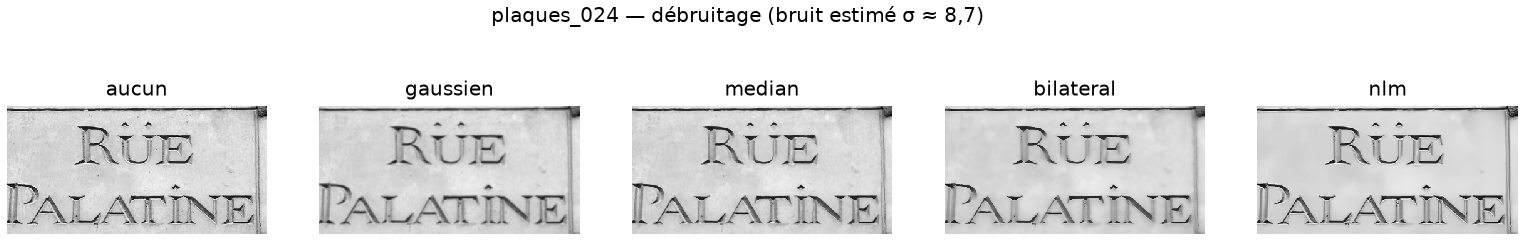
\includegraphics[width=0.92\linewidth]{debruitage_zoom_024.png}
\begin{itemize}\small
\item Bruit estimé automatiquement (Immerkær) $\Rightarrow$ force du filtre NLM adaptée
\item Bruit ajouté à 44 images propres : \alert{NLM} est le meilleur sur le bruit gaussien (SSIM 0,81), le \alert{médian} sur le poivre et sel (0,89)
\item CLAHE plutôt que l'égalisation globale : ombres et reflets
\item Sur l'image entière, le meilleur prétraitement (bilatéral + CLAHE) fait passer le F1 médian de 0,013 à 0,037 : la précision reste vers \alert{2\,\%}, car on améliore aussi les arbres
\end{itemize}
\end{frame}

% -----------------------------------------------------------------------------
\begin{frame}{Binarisation : globale ou adaptative}
\begin{columns}[c]
\column{0.6\textwidth}
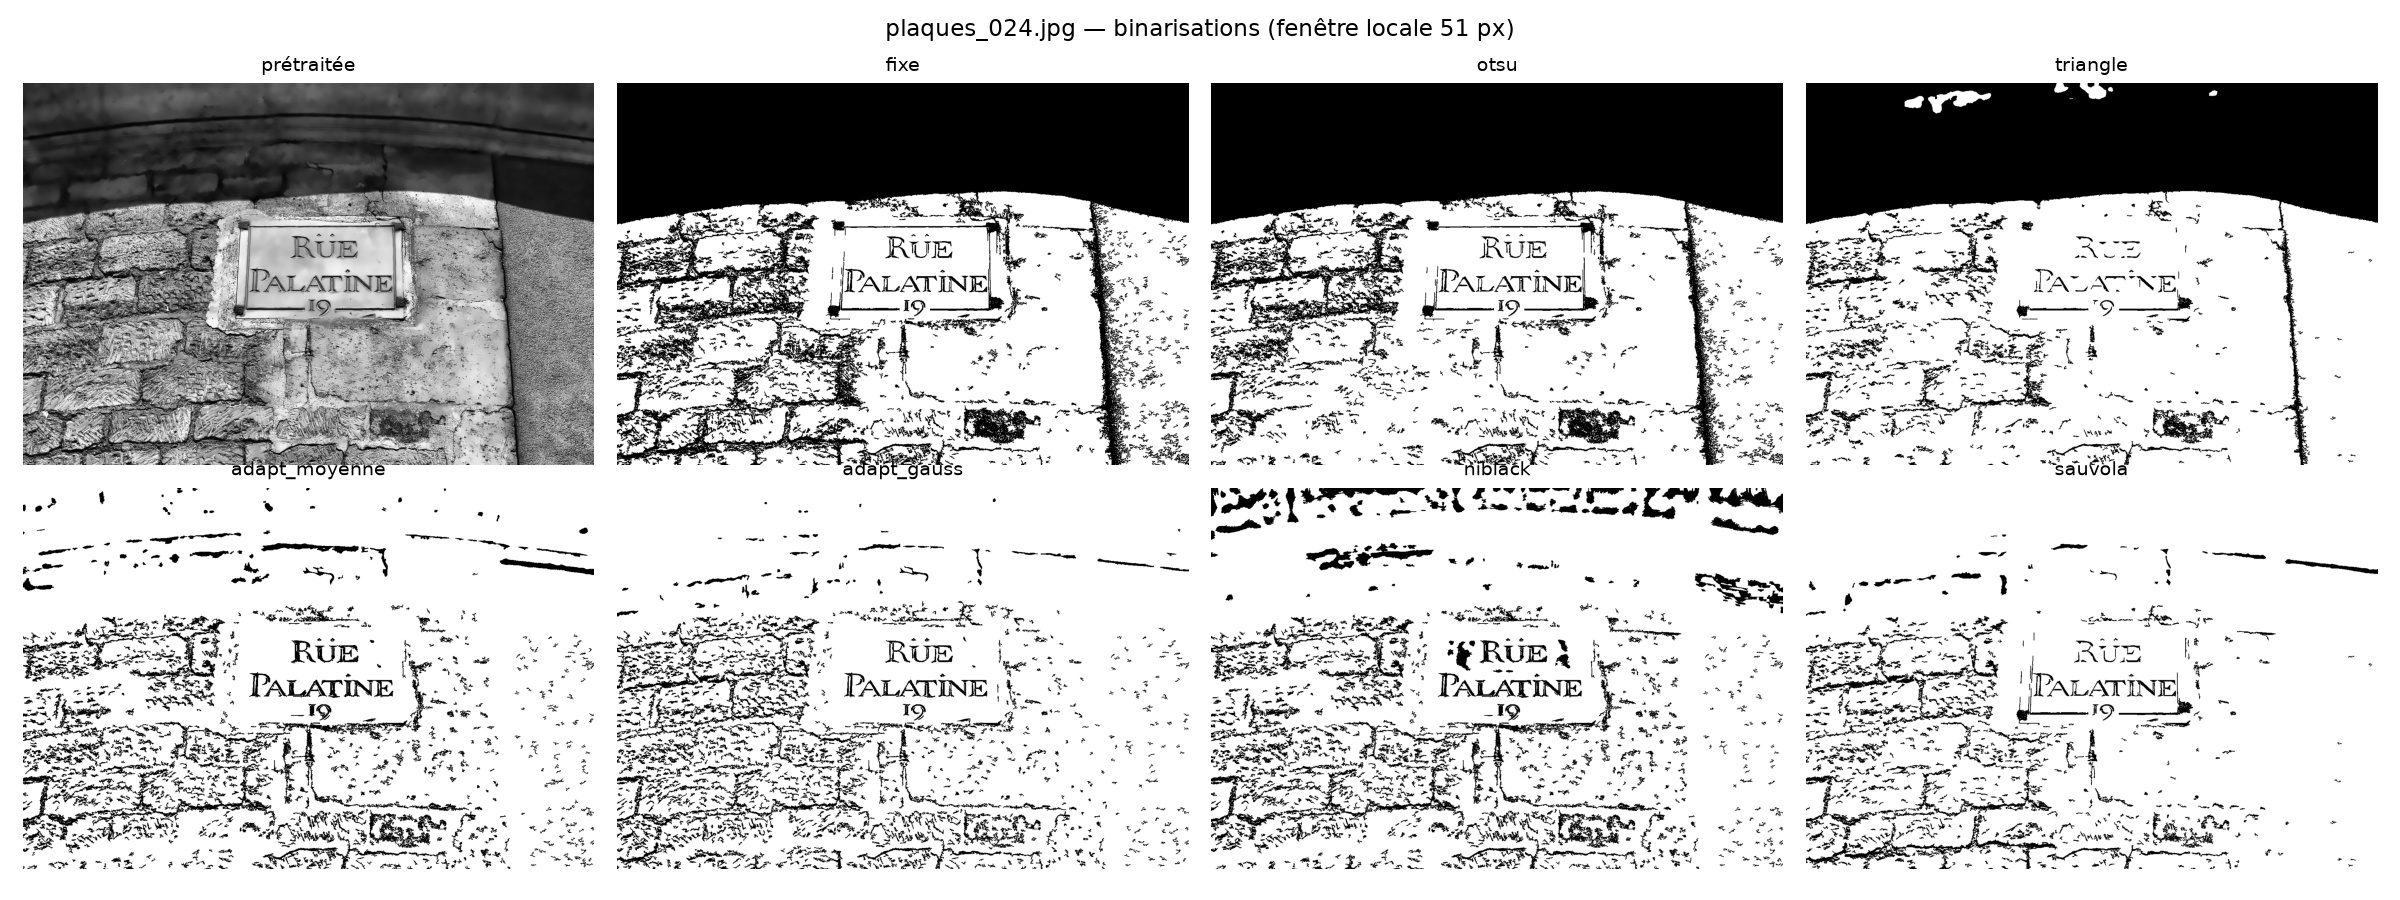
\includegraphics[width=\linewidth]{binarisation_024.png}
\column{0.38\textwidth}
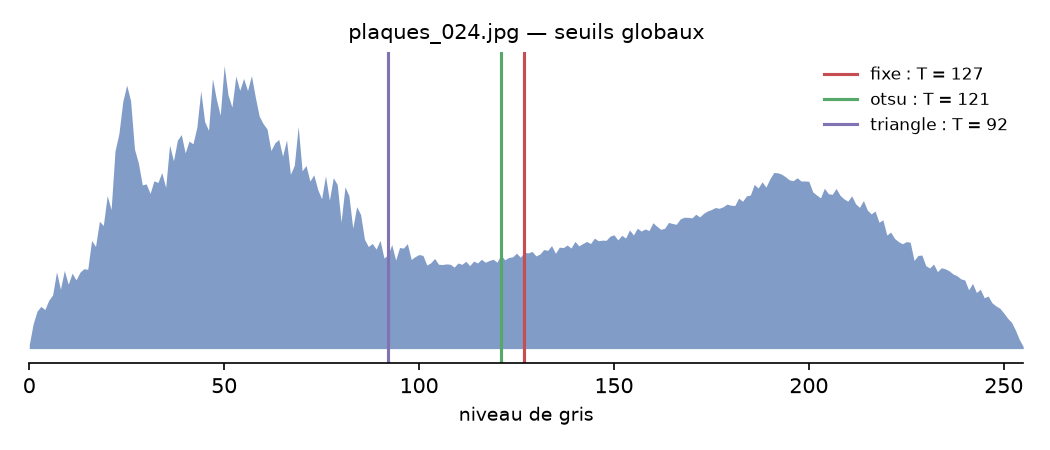
\includegraphics[width=\linewidth]{histogramme_024.png}
\end{columns}
\begin{itemize}\small
\item Ombre portée : les deux modes de l'histogramme sont l'\alert{ombre et la lumière}, pas le texte et le fond
\item Sur l'image entière, les méthodes adaptatives transforment la maçonnerie en traits : \alert{27 images sur 50 dégradées}
\item \textbf{Polarité} : le texte est la classe qui forme le plus d'objets de taille « caractère »
\item \textbf{Morphologie} : retirer les \alert{cadres} des plaques, sinon Tesseract ne lit \emph{rien}
\end{itemize}
\end{frame}

% -----------------------------------------------------------------------------
\begin{frame}{L'étape décisive : localiser le texte}
\begin{columns}[T]
\column{0.5\textwidth}
\textbf{Morphologie mathématique}
\begin{itemize}\small
\item gradient morphologique $\rightarrow$ bords
\item retrait des longs traits (cadres)
\item \alert{fermeture} horizontale : les lettres d'une ligne se rejoignent
\end{itemize}
\textbf{MSER}
\begin{itemize}\small
\item régions de forme stable quand le seuil varie
\item regroupées en lignes (hauteur, alignement, écart)
\end{itemize}
\textbf{Vérification commune}
\begin{itemize}\small
\item segmentation en caractères : $\ge 2$ composantes \alert{de même hauteur et alignées}
\item profil de projection pour séparer deux lignes
\item pyramide d'échelles
\end{itemize}
\column{0.48\textwidth}
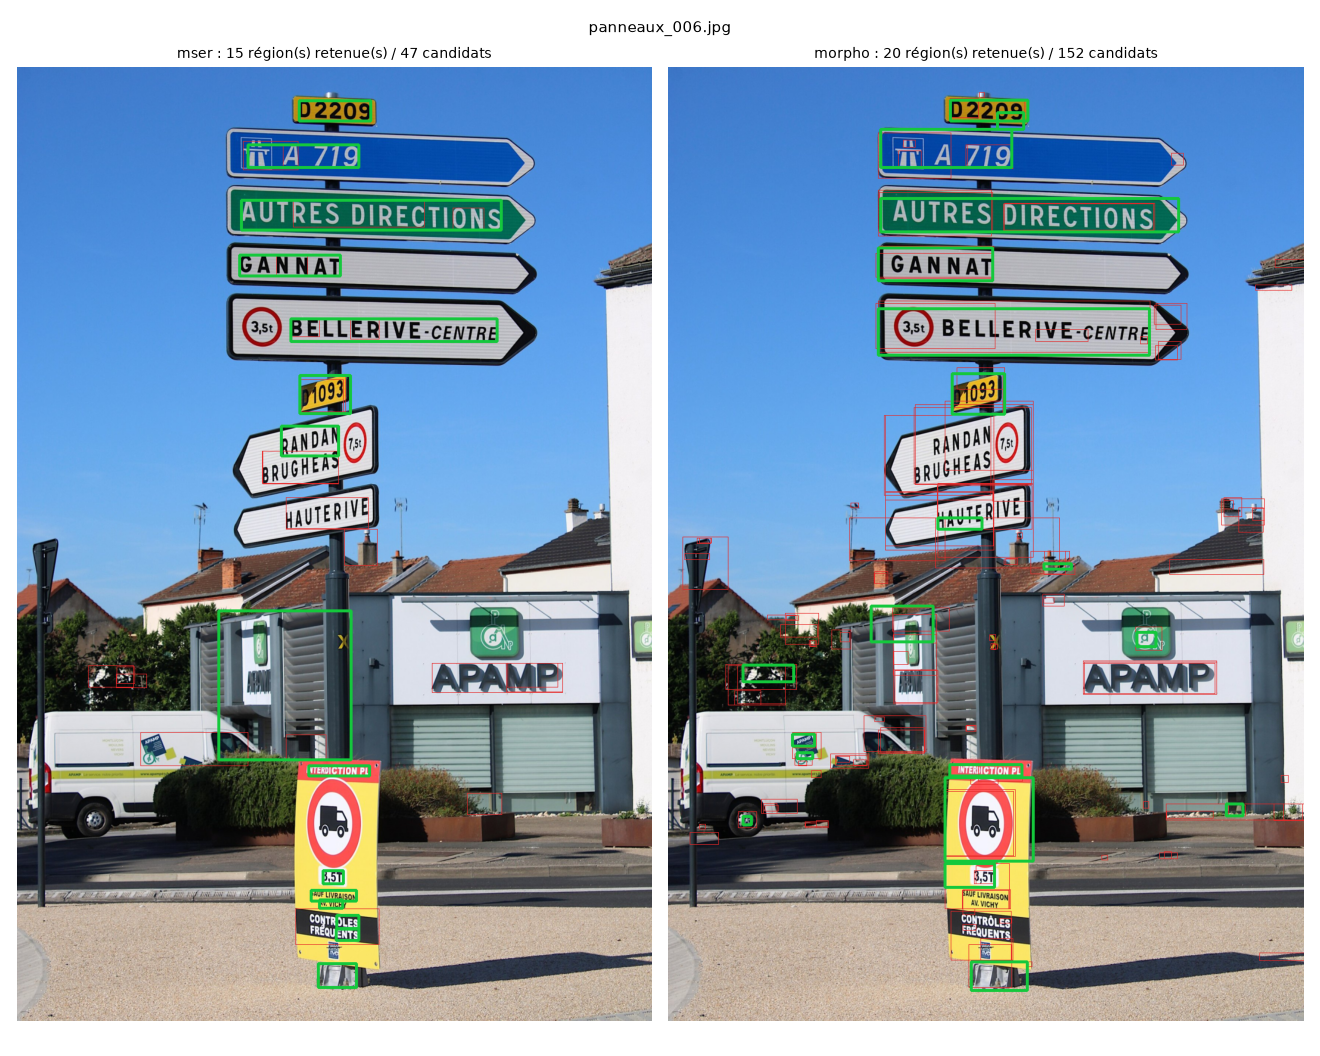
\includegraphics[width=\linewidth]{detection_006.png}
\vspace{0.2em}
{\scriptsize Rouge : candidats rejetés. Vert : zones retenues.}
\end{columns}
\end{frame}

% -----------------------------------------------------------------------------
\begin{frame}{Lire zone par zone}
\begin{columns}[c]
\column{0.55\textwidth}
\begin{enumerate}
\item recadrage avec une marge
\item mise à l'échelle : ligne de \alert{48 px}
\item binarisation de la zone seule
\item retrait des objets qui \alert{touchent le bord} (cadre, flèche)
\item Tesseract en mode « une ligne » (psm 7)
\item mots gardés si confiance $\ge 50$
\end{enumerate}
\vspace{0.6em}
Une fois la zone isolée, l'éclairage y est presque uniforme : un seuil global (Otsu) redevient adapté.
\column{0.4\textwidth}
\centering
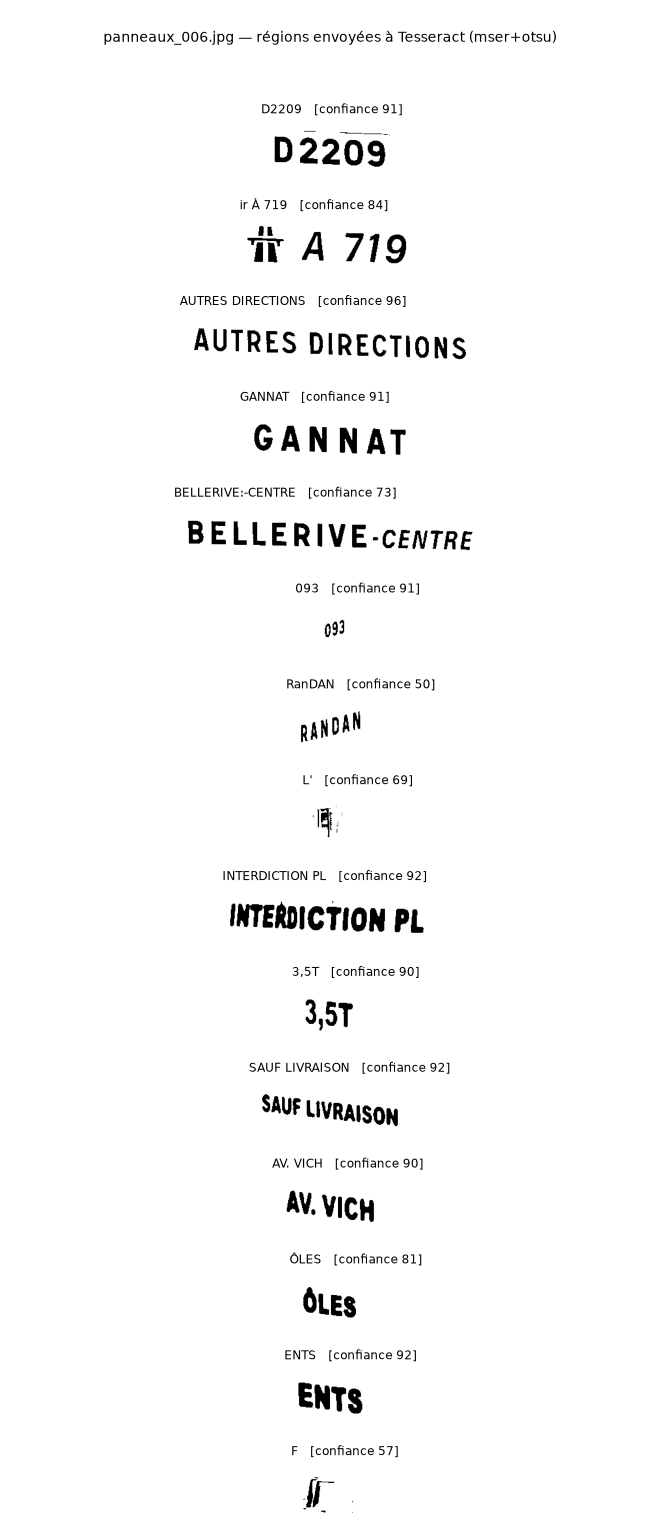
\includegraphics[height=0.78\textheight]{regions_006.png}
\end{columns}
\end{frame}

% -----------------------------------------------------------------------------
\begin{frame}{Résultats sur \nbImages{} images}
\tableauOuNote{tableau_principal.tex}{Lancer scripts/benchmark.py}
\vspace{-0.4em}
\begin{columns}[c]
\column{0.55\textwidth}
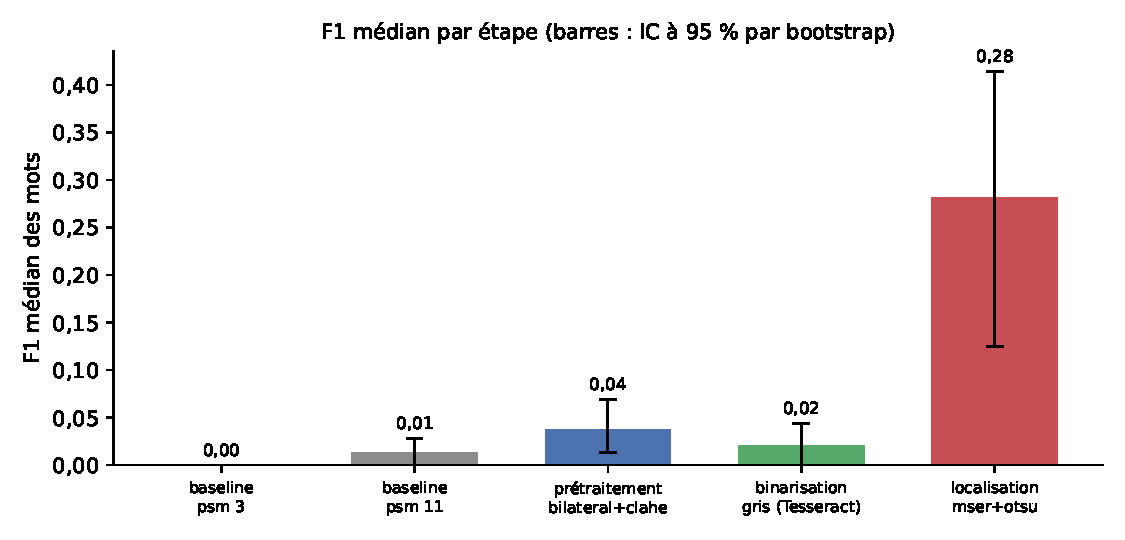
\includegraphics[width=\linewidth]{progression.pdf}
\column{0.43\textwidth}
\begin{itemize}\small
\item F1 médian : \alert{\baseFmed{} $\rightarrow$ \finFmed} (environ $\times$\facteurF)
\item \finMieux{} images améliorées, \finEgal{} égales, \finPire{} dégradées
\item Wilcoxon : $p$ \finP
\end{itemize}
\end{columns}
\end{frame}

% -----------------------------------------------------------------------------
\begin{frame}{Toutes les variantes de localisation}
\tableauOuNote{tableau_etape4.tex}{Lancer scripts/benchmark.py}
\vspace{-0.3em}
{\small F1 : médiane et IC à 95\,\% ; $+/=/-$ : images meilleures, égales, moins bonnes que la baseline ; $p$ : Wilcoxon apparié.}
\end{frame}

% -----------------------------------------------------------------------------
\begin{frame}{Quelle localisation, quelle binarisation ?}
\begin{columns}[c]
\column{0.45\textwidth}
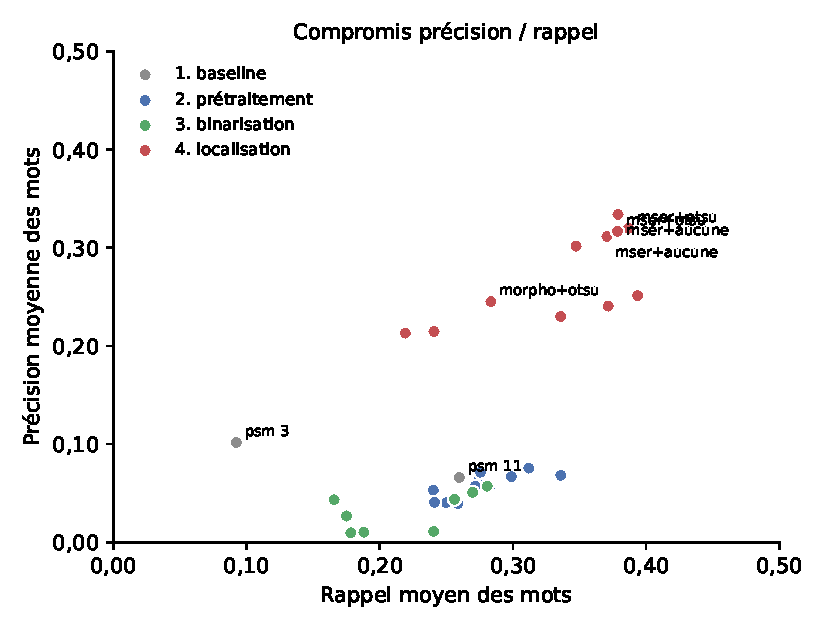
\includegraphics[width=\linewidth]{precision_rappel.pdf}
\column{0.53\textwidth}
\begin{itemize}\small
\item \alert{MSER bat la morphologie} : meilleur sur 28 images, moins bon sur 10 ; la morphologie s'accroche au feuillage
\item Combiner les deux n'apporte rien (plus de fausses zones)
\item Binarisation par zone (aucune, Otsu, Sauvola) : intervalles de confiance \alert{qui se recouvrent}
\item Version 2 (hauteur min. 0,5\,\%, 40 zones max.) : qualité inchangée ($p = 0{,}81$), pire temps \alert{49\,s $\rightarrow$ 19\,s}
\item Leçon : sur 6 images, la morphologie semblait meilleure $\Rightarrow$ ne pas régler sur quelques exemples
\end{itemize}
\end{columns}
\end{frame}

% -----------------------------------------------------------------------------
\begin{frame}{Par catégorie}
\centering
\tableauOuNote{tableau_categories.tex}{Lancer scripts/benchmark.py}
\begin{itemize}\small
\item Plaques et panneaux (42 images) : nets progrès en précision et en rappel
\item Affiches : la précision monte, le rappel baisse (polices décoratives, néons)
\item Numéros : 3 images, hors de portée
\end{itemize}
\end{frame}

% -----------------------------------------------------------------------------
\begin{frame}{Analyse des échecs : localisation ou reconnaissance ?}
\begin{columns}[c]
\column{0.55\textwidth}
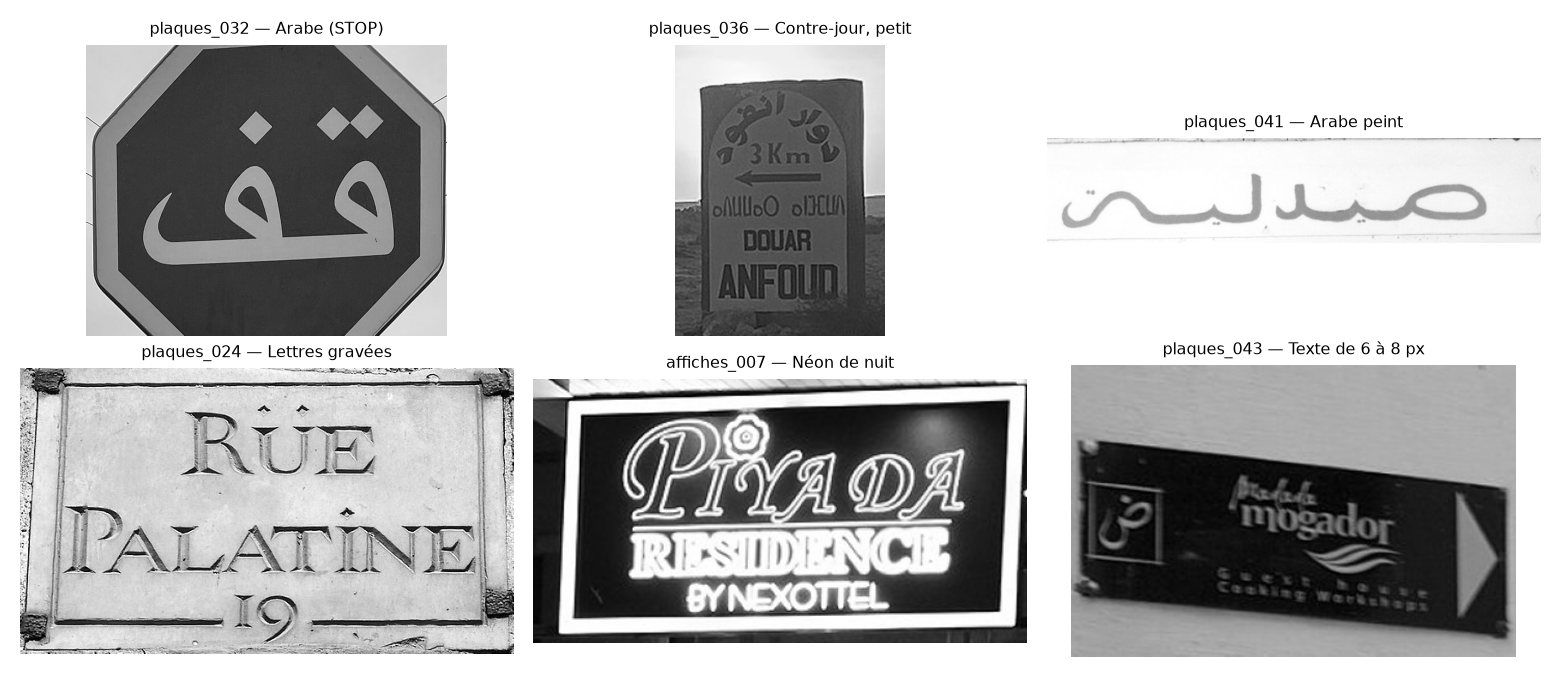
\includegraphics[width=\linewidth]{echecs.png}
\column{0.43\textwidth}
\small
Test : donner à Tesseract la zone \alert{recadrée à la main}
\begin{itemize}
\item lue $\Rightarrow$ échec de \textbf{localisation}, corrigeable : arabe (STOP), contre-jour, lettres blanches sur fond doré
\item non lue $\Rightarrow$ limite de la \textbf{reconnaissance} : arabe peint, néon, texte de 6 à 8 px
\end{itemize}
Corrections : hauteur minimale 0,5\,\%, plafond de 40 zones, canaux couleur et CLAHE en option
\end{columns}
\end{frame}

% -----------------------------------------------------------------------------
\begin{frame}{Restitution accessible}
\centering
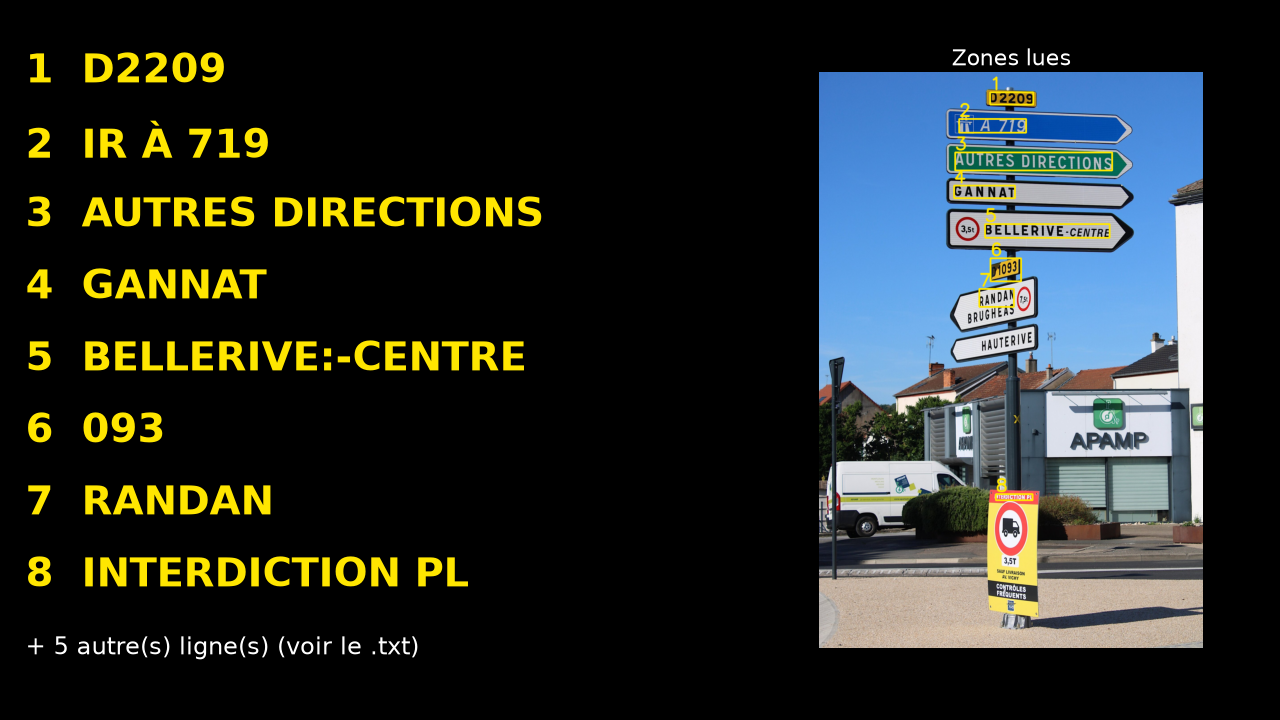
\includegraphics[width=0.72\linewidth]{carte_006.png}
\begin{itemize}\small
\item Jaune sur noir (contraste $\approx$ 17:1, niveau AAA des WCAG), très grand corps, une information par ligne
\item Zones numérotées sur la photo, pour qu'un accompagnant vérifie l'origine de chaque ligne ; texte brut pour une synthèse vocale
\end{itemize}
\end{frame}

% -----------------------------------------------------------------------------
\begin{frame}{Limites et perspectives}
\begin{columns}[T]
\column{0.48\textwidth}
\textbf{Limites}
\begin{itemize}\small
\item environ un mot sur trois retrouvé, un mot lu sur trois juste
\item écriture arabe, lettres gravées, néons, très petit texte
\item base de 50 images, petites catégories
\end{itemize}
\column{0.48\textwidth}
\textbf{Perspectives}
\begin{itemize}\small
\item vérification des lignes adaptée à l'arabe + langue \texttt{ara}
\item détecteurs appris (EAST, CRAFT) : module remplaçable
\item synthèse vocale
\item temps réel : ne lire que la zone visée
\end{itemize}
\end{columns}
\end{frame}

% -----------------------------------------------------------------------------
\begin{frame}{Conclusion}
\begin{itemize}
\item Un pipeline complet, de la photo à la restitution accessible
\item Mesurer chaque étape a montré que \alert{la localisation est décisive}, pas l'amélioration de l'image entière
\item F1 médian : \gros{\baseFmed} $\rightarrow$ \gros{\finFmed}, amélioration significative sur \finMieux{}/\nbImages{} images
\item Une analyse des échecs qui sépare localisation et reconnaissance, et fixe les priorités
\end{itemize}
\vfill
\centering
\texttt{uv run scripts/lire\_image.py photo.jpg --carte carte.png}
\end{frame}

\end{document}
